\documentclass{article}
\usepackage[preprint]{neurips_2024}
\usepackage[utf8]{inputenc}
\usepackage[T1]{fontenc}
\usepackage[colorlinks=true,linkcolor=black,citecolor=blue!50!black,urlcolor=blue!50!black]{hyperref}
\usepackage{url}
\usepackage{booktabs}
\usepackage{amsmath,amssymb,amsthm}
\usepackage{microtype}
\usepackage{xcolor}
\usepackage{tikz}
\usetikzlibrary{arrows.meta,positioning}

\newtheorem{proposition}{Proposition}
\newtheorem{lemma}{Lemma}
\theoremstyle{definition}
\newtheorem{definition}{Definition}
\newtheorem{assumption}{Assumption}

\newcommand{\E}{\mathbb{E}}
\newcommand{\dE}{\Delta E}
\newcommand{\dP}{\Delta P}

\title{The State Defect, Plasticity, Empowerment and the Return}

\author{Zihan Wang\\ Mila, McGill University}

\begin{document}
\maketitle

\begin{abstract}
A small agent in a large world keeps a memory that merges histories.
We measure what the memory loses by the state defect, the information the history still carries about the next observation beyond the memory and the action, and split it in two ways into four terms.
Two of the terms are differences between plasticity and empowerment measured at the history and at the memory.
This note collects the definitions and exact identities and derives, step by step, how the defect bounds the error of the value the memory can represent.
How the four terms enter the return is left open and is the subject of the next steps.
\end{abstract}

\section{Setting}

\begin{center}
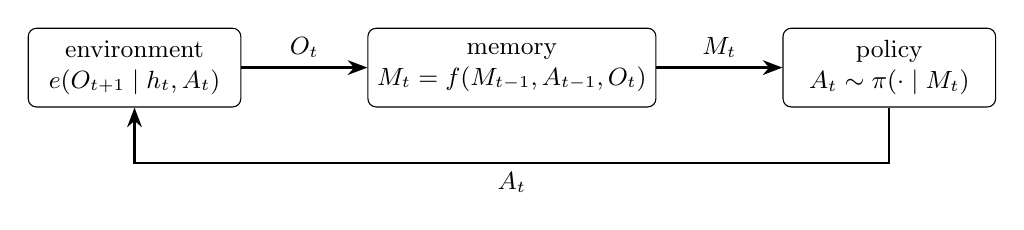
\begin{tikzpicture}[>={Stealth[length=2.5mm]}, node distance=10mm and 16mm,
  box/.style={draw, rounded corners=3pt, minimum height=10mm, minimum width=27mm, align=center, font=\small}]
\node[box] (world) {environment\\ $e(O_{t+1}\mid h_t, A_t)$};
\node[box, right=of world] (mem) {memory\\ $M_t = f(M_{t-1}, A_{t-1}, O_t)$};
\node[box, right=of mem] (pol) {policy\\ $A_t \sim \pi(\cdot \mid M_t)$};
\draw[->, thick] (world) -- node[above, font=\small] {$O_t$} (mem);
\draw[->, thick] (mem) -- node[above, font=\small] {$M_t$} (pol);
\draw[->, thick] (pol.south) -- ++(0,-7mm) -| node[pos=0.25, below, font=\small] {$A_t$} (world.south);
\end{tikzpicture}
\end{center}

The history is $h_t=(O_{1:t},A_{1:t-1})$, and the reward $R_t$ is one component of the observation $O_t$.

\begin{assumption}[Environment]\label{as:env}
The environment $e(O_{t+1}\mid h_t,A_t)$ may depend on the whole history. No Markov or stationarity assumption is made; a changing environment is one such law.
\end{assumption}

\begin{assumption}[Memory]\label{as:mem}
The memory is updated recursively, $M_{t+1}=f(M_t,A_t,O_{t+1})$. Hence $M_t$ is a deterministic function of $h_t$.
\end{assumption}

\begin{assumption}[Policy]\label{as:pol}
The action depends on the history only through the memory: $A_t\sim\pi(\cdot\mid M_t)$, with randomness independent of everything else. In particular $I(h_t;A_t\mid M_t)=0$.
\end{assumption}

Observation and action sets are finite, rewards lie in an interval of length $\Delta R$, and all probabilities are under the distribution induced by the environment, the memory and the policy.

\section{The state defect}

\begin{definition}
The state defect is
\[
D_t \;=\; I\big(h_t;O_{t+1}\mid M_t,A_t\big)\;=\;\E\left[\log\frac{p(O_{t+1}\mid h_t,A_t)}{p(O_{t+1}\mid M_t,A_t)}\right].
\]
\end{definition}

$D_t$ is the expected gain in log-likelihood from predicting the next observation with the whole history instead of the memory. $D_t=0$ if and only if any two histories with the same memory value give the same distribution of $O_{t+1}$, for every action the agent takes there. The condition concerns the pairs $(h_t,a)$ that occur under the agent's own behaviour.

\section{Plasticity and empowerment at the history and at the memory}

\citet{abel2025plasticity} define, in one-step form, the empowerment of the action over the next observation and the plasticity of the next action to the observation,
\[
E_t=I(A_t;O_{t+1}\mid h_t),\qquad P_{t+1}=I(O_{t+1};A_{t+1}\mid h_t,A_t).
\]
The agent cannot condition on the full history. The same quantities computed from the memory are
\[
E_t(M)=I(A_t;O_{t+1}\mid M_t),\qquad P_{t+1}(M)=I(O_{t+1};A_{t+1}\mid M_t,A_t).
\]

\begin{proposition}[The two mismatches]\label{prop:mismatch}
Under Assumptions~\ref{as:mem} and~\ref{as:pol},
\[
\begin{aligned}
\dE_t&=E_t-E_t(M)=I(h_t;A_t\mid M_t,O_{t+1})\ge0,\\
\dP_t&=P_{t+1}(M)-P_{t+1}=I(h_t;A_{t+1}\mid M_t,A_t)\ge0 .
\end{aligned}
\]
\end{proposition}

\begin{proof}
Write each mutual information as a difference of conditional entropies. For empowerment, $H(A_t\mid h_t)=H(A_t\mid M_t)$ by Assumption~\ref{as:pol}, so $\dE_t=H(A_t\mid M_t,O_{t+1})-H(A_t\mid h_t,O_{t+1})$, which is $I(h_t;A_t\mid M_t,O_{t+1})$ because $M_t$ is a function of $h_t$. For plasticity, $H(A_{t+1}\mid h_t,A_t,O_{t+1})$ and $H(A_{t+1}\mid M_t,A_t,O_{t+1})$ both equal $H(A_{t+1}\mid M_{t+1})$, since $M_{t+1}=f(M_t,A_t,O_{t+1})$ and $A_{t+1}$ depends only on $M_{t+1}$; subtracting gives $\dP_t=H(A_{t+1}\mid M_t,A_t)-H(A_{t+1}\mid h_t,A_t)=I(h_t;A_{t+1}\mid M_t,A_t)$.
\end{proof}

The memory can only under-estimate empowerment and over-estimate plasticity. Two bounds follow directly: $\dE_t\le H(A_t\mid M_t)$, so $\dE_t=0$ under a policy that puts all probability on one action at $M_t$; and $\dP_t\le P_{t+1}(M)$, so $\dP_t=0$ when $A_{t+1}$ does not depend on $O_{t+1}$ given $(M_t,A_t)$, for example under the uniform policy.

\section{Two splits of the defect}

\begin{proposition}[Four terms]\label{prop:splits}
Under Assumptions~\ref{as:mem} and~\ref{as:pol},
\[
D_t\;=\;\underbrace{I(h_t;O_{t+1}\mid M_t)}_{D^0_t}+\dE_t\;=\;\dP_t+\underbrace{I(h_t;O_{t+1}\mid M_t,A_t,A_{t+1})}_{D^+_t}.
\]
\end{proposition}

\begin{proof}
By the chain rule, $I(h_t;O_{t+1},A_t\mid M_t)=I(h_t;A_t\mid M_t)+D_t=D^0_t+\dE_t$, and the first term is zero. Again, $I(h_t;O_{t+1},A_{t+1}\mid M_t,A_t)=D_t+I(h_t;A_{t+1}\mid M_t,A_t,O_{t+1})=\dP_t+D^+_t$, and the middle term is zero as in the proof of Proposition~\ref{prop:mismatch}.
\end{proof}

$D^0_t$ is what the next observation reveals about the dropped part of the history without the action, and $\dE_t$ what it reveals only when read together with the action. $\dP_t$ is the part the next action depends on, and $D^+_t$ the part it does not.

\section{Every term with the reward separated}

Write the next observation as $O_{t+1}=(R_{t+1},\bar O_{t+1})$, the reward and the rest. We split each of the four terms into a reward part and a rest part, using only the chain rule, and keep track of which parts are nonnegative.

\subsection{The defect}
By the chain rule on $O_{t+1}=(R_{t+1},\bar O_{t+1})$,
\[
D_t=\underbrace{I(h_t;R_{t+1}\mid M_t,A_t)}_{D^R_t}+\underbrace{I(h_t;\bar O_{t+1}\mid M_t,A_t,R_{t+1})}_{D^{\bar O}_t}.
\]

\subsection{$D^0$ and $D^+$}
By the same chain rule inside $D^0_t$ and $D^+_t$,
\begin{align*}
D^0_t&=\underbrace{I(h_t;R_{t+1}\mid M_t)}_{D^{0,R}_t}+\underbrace{I(h_t;\bar O_{t+1}\mid M_t,R_{t+1})}_{D^{0,\bar O}_t},\\
D^+_t&=\underbrace{I(h_t;R_{t+1}\mid M_t,A_t,A_{t+1})}_{D^{+,R}_t}+\underbrace{I(h_t;\bar O_{t+1}\mid M_t,A_t,A_{t+1},R_{t+1})}_{D^{+,\bar O}_t}.
\end{align*}
All four parts are mutual informations, hence nonnegative.

\subsection{$\dE$}
Expand $I(h_t;R_{t+1},A_t\mid M_t)$ in two orders. Since $I(h_t;A_t\mid M_t)=0$,
\[
D^R_t=D^{0,R}_t+\underbrace{I(h_t;A_t\mid M_t,R_{t+1})}_{\dE^R_t}.
\]
Expand $I(h_t;\bar O_{t+1},A_t\mid M_t,R_{t+1})$ in two orders:
\[
\dE^R_t+D^{\bar O}_t=D^{0,\bar O}_t+\dE_t .
\]
Define $\dE^{\bar O}_t=\dE_t-\dE^R_t$. Then
\begin{gather*}
\dE_t=\dE^R_t+\dE^{\bar O}_t,\qquad D^{\bar O}_t=D^{0,\bar O}_t+\dE^{\bar O}_t,\\
\dE^{\bar O}_t=I(h_t;A_t\mid M_t,R_{t+1},\bar O_{t+1})-I(h_t;A_t\mid M_t,R_{t+1}).
\end{gather*}
$\dE^R_t\ge0$, but $\dE^{\bar O}_t$ is a difference of two mutual informations and can be negative.

\subsection{$\dP$}
Expand $I(h_t;R_{t+1},A_{t+1}\mid M_t,A_t)$ in two orders:
\[
D^R_t+\underbrace{I(h_t;A_{t+1}\mid M_t,A_t,R_{t+1})}_{\dP^{\bar O}_t}=\dP_t+D^{+,R}_t .
\]
Define $\dP^R_t=\dP_t-\dP^{\bar O}_t$. Then
\begin{gather*}
\dP_t=\dP^R_t+\dP^{\bar O}_t,\qquad D^R_t=\dP^R_t+D^{+,R}_t,\\
\dP^R_t=I(h_t;R_{t+1}\mid M_t,A_t)-I(h_t;R_{t+1}\mid M_t,A_t,A_{t+1}),
\end{gather*}
and, subtracting from Proposition~\ref{prop:splits}, $D^{\bar O}_t=\dP^{\bar O}_t+D^{+,\bar O}_t$.
$\dP^{\bar O}_t\ge0$: it is the dependence of the next action on the history beyond the memory once the reward is known, which can only come through $\bar O_{t+1}$. $\dP^R_t$ is a difference of two mutual informations and can be negative.

\subsection{The full table}

\begin{proposition}[Reward-separated splits]\label{prop:table}
Under Assumptions~\ref{as:mem} and~\ref{as:pol},
\begin{align*}
D^R_t&=D^{0,R}_t+\dE^R_t=\dP^R_t+D^{+,R}_t,\\
D^{\bar O}_t&=D^{0,\bar O}_t+\dE^{\bar O}_t=\dP^{\bar O}_t+D^{+,\bar O}_t,
\end{align*}
and each of the four terms of Proposition~\ref{prop:splits} is the sum of its reward part and its rest part. All parts are nonnegative except $\dE^{\bar O}_t$ and $\dP^R_t$.
\end{proposition}

\subsection{The reward parts are reward empowerment and reward plasticity}

Define the empowerment of the action over the reward and the plasticity of the next action to the reward, at the history and at the memory:
\begin{gather*}
E^R_t=I(A_t;R_{t+1}\mid h_t),\qquad E^R_t(M)=I(A_t;R_{t+1}\mid M_t),\\
P^R_{t+1}=I(R_{t+1};A_{t+1}\mid h_t,A_t),\qquad P^R_{t+1}(M)=I(R_{t+1};A_{t+1}\mid M_t,A_t).
\end{gather*}

\begin{proposition}\label{prop:reward-pe}
Under Assumptions~\ref{as:mem} and~\ref{as:pol},
\[
\dE^R_t=E^R_t-E^R_t(M),\qquad \dP^R_t=P^R_{t+1}(M)-P^R_{t+1},
\]
so
\[
D^R_t=D^{0,R}_t+\big(E^R_t-E^R_t(M)\big)=\big(P^R_{t+1}(M)-P^R_{t+1}\big)+D^{+,R}_t .
\]
\end{proposition}

\begin{proof}
Expand $I(A_t;R_{t+1},h_t\mid M_t)$ in two orders: $E^R_t(M)+I(A_t;h_t\mid M_t,R_{t+1})=I(A_t;h_t\mid M_t)+I(A_t;R_{t+1}\mid h_t)=0+E^R_t$, using that $M_t$ is a function of $h_t$. For plasticity, expand $I(R_{t+1};A_{t+1},h_t\mid M_t,A_t)$ in two orders: $P^R_{t+1}(M)+I(R_{t+1};h_t\mid M_t,A_t,A_{t+1})=I(R_{t+1};h_t\mid M_t,A_t)+P^R_{t+1}$, that is $P^R_{t+1}(M)-P^R_{t+1}=D^R_t-D^{+,R}_t=\dP^R_t$.
\end{proof}

\paragraph{Two observations.}
\begin{enumerate}
\item \emph{The memory can over- or under-estimate reward plasticity.} For the whole observation, $\dP_t\ge0$: the memory can only over-estimate plasticity (Proposition~\ref{prop:mismatch}). For the reward alone, $\dP^R_t$ can be negative. The proof of $\dP_t\ge0$ used that $A_{t+1}$ is independent of the history given $(M_t,A_t,O_{t+1})$; given $(M_t,A_t,R_{t+1})$ alone this fails, because the next action also responds to $\bar O_{t+1}$, which carries information about the history. For example, if $R_{t+1}$ is a fair coin independent of the history, $\bar O_{t+1}=R_{t+1}\oplus c$ for a bit $c$ in the dropped history, and the next action copies $\bar O_{t+1}$, then $D^R_t=0$ but $D^{+,R}_t=1$ bit, so $\dP^R_t=-1$ bit.
\item \emph{$\dE_t=0$ does not mean that the reward has no action-dependent hidden part.} $\dE_t=\dE^R_t+\dE^{\bar O}_t$, and $\dE^{\bar O}_t$ can be negative. If the observation shows the action just taken ($A_t$ is a component of $\bar O_{t+1}$), then $\dE_t=I(h_t;A_t\mid M_t,O_{t+1})=0$, while $\dE^R_t=I(h_t;A_t\mid M_t,R_{t+1})$ can be positive; the corresponding information is then counted in $D^{0,\bar O}_t$, and $\dE^{\bar O}_t=-\dE^R_t$. For example, if a hidden variable $c$ in the dropped history decides which of two actions is rewarded, $R_{t+1}=\mathbf 1\{A_t=c\}$, and the policy is uniform, then $\dE^R_t=1$ bit and $D^{0,R}_t=0$, whether or not the observation shows the action. A measured $\dE_t\approx0$ in a world whose observation shows the agent's own move therefore says nothing about $\dE^R_t$; the reward part has to be measured on its own.
\end{enumerate}

\section{From the reward parts to the return}

We use three facts: (F1) $h_{t+1}=(h_t,A_t,O_{t+1})$ and $M_t$ is a function of $h_t$; (F2) $M_{t+1}=f(M_t,A_t,O_{t+1})$; (F3) $A_{t+1}$ depends on the past only through $M_{t+1}$. From (F2) and (F3), for any variables $V$ from the past,
\begin{equation}\label{eq:action-zero}
I(V;A_{t+1}\mid M_t,A_t,O_{t+1})=0 .
\end{equation}

\subsection{Step 1: the next reward}

Fix $(m,a)$. The expected next reward the agent can estimate is the average over the histories behind $m$, $\E[R_{t+1}\mid M_t=m,A_t=a]=\sum_hP(h_t=h\mid M_t=m)\,\E[R_{t+1}\mid h_t=h,A_t=a]$, using (F3). For one history $h$, let $P_h=P(R_{t+1}\mid h_t=h,A_t=a)$ and $Q=P(R_{t+1}\mid M_t=m,A_t=a)$.
\begin{enumerate}
\item $|\E_{P_h}R-\E_QR|\le\Delta R\cdot\mathrm{TV}(P_h,Q)$, since $\E_{P_h}R-\E_QR=\sum_r(P_h(r)-Q(r))(r-c)$ for the midpoint $c$ of the reward range.
\item $\mathrm{TV}(P_h,Q)\le\sqrt{\mathrm{KL}(P_h\|Q)/2}$ (Pinsker).
\item Average over $h$ behind $m$ and over $(M_t,A_t)$ with Jensen's inequality; the average of $\mathrm{KL}(P_h\|Q)$ is $D^R_t$.
\end{enumerate}
Hence, with Propositions~\ref{prop:table} and~\ref{prop:reward-pe},
\[
\E\big|\E[R_{t+1}\mid h_t,A_t]-\E[R_{t+1}\mid M_t,A_t]\big|\le\Delta R\sqrt{D^R_t/2},\qquad D^R_t=D^{0,R}_t+\dE^R_t=\dP^R_t+D^{+,R}_t .
\]

\subsection{Step 2: the reward two steps later}

\begin{enumerate}
\item $R_{t+2}$ is a component of $O_{t+2}$, so by data processing $I(h_t;R_{t+2}\mid M_t,A_t)\le I(h_t;O_{t+1},A_{t+1},R_{t+2}\mid M_t,A_t)$.
\item Chain rule in the order $O_{t+1}$, $A_{t+1}$, $R_{t+2}$; the middle term is zero by \eqref{eq:action-zero}:
\[
I(h_t;O_{t+1},A_{t+1},R_{t+2}\mid M_t,A_t)=D_t+L^R_{t+1},
\]
with $L^R_{t+1}=I(h_t;R_{t+2}\mid M_t,A_t,O_{t+1},A_{t+1})$.
\item By (F1), $h_{t+1}$ carries the same information as $(h_t,M_t,A_t,O_{t+1})$. The chain rule, first $(M_t,A_t,O_{t+1})$ and then $h_t$, and (F2) to remove $M_{t+1}$ from the second condition, give
\[
D^R_{t+1}=I(M_t,A_t,O_{t+1};R_{t+2}\mid M_{t+1},A_{t+1})+L^R_{t+1}.
\]
The first term is what the update $f$ at $t+1$ discards that still predicts $R_{t+2}$; $L^R_{t+1}$ is what was lost before. Both are nonnegative, so $L^R_{t+1}\le D^R_{t+1}$.
\end{enumerate}
Hence
\[
I(h_t;R_{t+2}\mid M_t,A_t)\le D_t+D^R_{t+1}.
\]
At $t+1$ only the reward part enters. At $t$ the whole defect enters, $D_t=D^R_t+D^{\bar O}_t$, because the reward at $t+2$ can depend on the rest of the observation at $t+1$, through the environment and through the next action.

\subsection{Step 3: $k$ steps and the infinite horizon}

Let $Z_{t,k}=(M_t,A_t,O_{t+1},A_{t+1},\dots,O_{t+k},A_{t+k})$. Repeating Step~2,
\[
I(h_t;R_{t+k+1}\mid M_t,A_t)\le\sum_{j=0}^{k-1}I(h_t;O_{t+j+1}\mid Z_{t,j})+I(h_t;R_{t+k+1}\mid Z_{t,k})\le\sum_{j=0}^{k-1}D_{t+j}+D^R_{t+k}.
\]
Every action term vanishes because $M_{t+j}$ is a function of the earlier variables in $Z_{t,j}$, and each remaining term is bounded as in Step~2(3) at the corresponding time.
With $\gamma<1$, $q_\pi(h,a)=\E[\sum_{k\ge0}\gamma^kR_{t+k+1}\mid h_t=h,A_t=a]$ and $q_\pi(m,a)=\E[q_\pi(h_t,a)\mid M_t=m]$, writing the difference as a discounted sum of reward differences and bounding each as in Step~1,
\[
\E\big|q_\pi(h_t,A_t)-q_\pi(M_t,A_t)\big|\le\Delta R\sum_{k\ge0}\gamma^k\sqrt{\tfrac12\Big(\sum_{j=0}^{k-1}D_{t+j}+D^R_{t+k}\Big)} .
\]
If $D_{t+j}\le\bar D$ for all $j$, the bracket is at most $(k+1)\bar D$, and $\sum_{k\ge0}\gamma^k\sqrt{k+1}\le\sqrt{\sum_k\gamma^k}\sqrt{\sum_k\gamma^k(k+1)}=(1-\gamma)^{-3/2}$ (Cauchy--Schwarz), so the error is at most $\Delta R\sqrt{\bar D/2}\,(1-\gamma)^{-3/2}$. The structure is that of the approximate information state of \citet{subramanian2022approximate}. The reward-separated splits and the split of Step~2(3) have not been checked against the literature.

\section{Open questions}

\begin{enumerate}
\item The bounds of Section~6 concern the value. Policy improvement needs the advantage, which subtracts the part that does not depend on the action. How do the four terms enter the error of the advantage?
\item In Step~2 of Section~6 the whole defect at $t$ enters. Which part of $D^0_t,\dE_t,\dP_t,D^+_t$ actually reaches later rewards, through the environment and through the agent's own actions?
\item In continual RL the policy keeps changing. How do $\dE$ and $\dP$ change along the learning path, and what does that imply for what the memory should keep?
\end{enumerate}

\bibliographystyle{plainnat}
\bibliography{references}

\end{document}
